\chapter{Inductive Reasoning with \textsc{KANDY}}\label{chap:kandyind}
In this chapter we evaluate {\it neural} and {\it symbolic} approaches against the two \textsc{KANDY-Induction} curricula. In these curricula, the binary classification task can only be solved successfully by agents capable of extracting First-order rules from observations.
The content of this chapter is based on our MLJ journal paper~\cite{lorello2025kandy}.

\section{Neural Experiments}\label{sec:kandy:neur-exp}
We evaluate Neural Networks with respect to their ability to solve the binary classification problems of \textsc{KANDY-Induction}, as a proxy for their sub-symbolic inductive capabilities. The architecture for each experiment consists in a neural backbone $\phi_\vtheta: \sX \mapsto \R^d$, mapping the input image to a latent representation, and one or more classification heads $\psi_{\vtheta'}: \R^d \mapsto [0, 1]$.
We consider the following models as a representative sample of the most widely employed architectures for image classification: (i.) \textit{Multi-layer Perceptrons}, (ii.) \textit{Convolutional Neural Networks}, (iii, iv.) \textit{Residual Networks}~\cite{he2016deep}, and (v.) \textit{Vision Transformers}~\cite{dosovitskiy2020image}.
The effect of time on the learning process is addressed by exploring four different learning settings: (i.) \textit{Independent}, (ii.) \textit{Joint}, (iii.) \textit{Task-incremental}, (iv.) \textit{Continual online}.
Training is performed while sampling positive/negative training data in a class-balanced manner (for each task), thus possibly repeating examples of the least represented category. 
Continual Learning settings are tackled using Experience Replay with Class-balanced Reservoir Sampling~\cite{chrysakis2020online}. The main hyper-parameters are cross-validated by exhaustively searching on fixed grids of values (Appendix~\ref{app:kandyhyper}).

\paragraph{Architectures.} The Multi-layer perceptron (\textsc{MLP}) backbone ($\phi$) consists of a hidden layer with 100 neurons followed by hyperbolic tangent activations, while the Convolutional Neural Network (\textsc{CNN}) backbone is the following architecture:
\begin{verbatim}
Conv2D(features=64, kernel=(5,5), stride=1)
MaxPooling2D()
ReLU()
Conv2D(features=128, kernel=(3,3), stride=2)
MaxPooling2D()
ReLU()
Conv2D(features=256, kernel=(3,3), stride=2)
MaxPooling2D()
Flatten()
Linear(in=5*5*256, out=4096)
Dropout(p=0.1)
\end{verbatim}
Backbones \textsc{ResNet-50} and \textsc{ResNet-50 (H)} are residual networks, where the last layer computes a 4096-dimensional embedding. The former is trained from scratch at each layer, while the latter is initialized with pre-trained weights (ImageNet) and every layer, except the last one, is frozen during training.
Similarly, backbone \textsc{ViT-16 (H)} is a Vision Transformer pre-trained on ImageNet and frozen, with the exception of the last layer.
For every architecture, classification heads ($\psi$) are linear layers with one neuron for each task, equipped with sigmoid activations. 

\paragraph{Learning Settings.} In the \textit{Independent} learning setting, each task is observed in isolation, and the architecture is composed of a single classification head $\psi_{\vtheta'}$, which is re-initialized along with the backbone and trained independently, for each task within the curriculum. This setting corresponds to the baseline performance expected when there is no interaction across tasks.
The architecture implementing the other learning settings is composed of a single backbone, equipped with different classification heads $\psi^{(t)}_{\vtheta'}$ (one for each task in the curriculum). For each of the learning settings, both training and inference data points are annotated with a task-id $t$, to select the correct prediction.\footnote{i.e., $\evy[t] = \psi^{(t)}_{\vtheta'}(\phi^{(t)}_{\vtheta}(\vx))$ for the Independent case, $\evy[t] = \psi^{(t)}_{\vtheta'}(\phi_\vtheta(\vx))$ for every other.}
The \textit{Joint} learning setting is a classic instance of Multi-task Learning, where the whole training data is shuffled and used to optimize both $\phi_\vtheta$ and $\psi^{(t)}_{\vtheta'}$ at once. In this setting, internal representations and weights are shared across each task, without any information loss caused by temporal dynamics.
\textit{Task-incremental} and \textit{Continual online} learning are two instances of Continual Learning, where the architecture observes one task at the time (i.e., for task $t$, we train $\phi_{t;\vtheta} \circ \psi^{(t)}_{\vtheta'}$ and freeze every $\psi^{(t')}$ for $t' \not = t$). In these settings temporal dynamics are expected to cause catastrophic forgetting, but also to guide the learning process thanks to the curricular nature of \textsc{KANDY}.
The \textit{Task-incremental} learning setting allows to shuffle data within a single task and to perform multiple epochs of training, while the \textit{Continual online} learning setting is characterized by a single pass, without altering the order of samples within the dataset.
For each experiment we measure \textsc{Average Accuracy}, \textsc{Average Forgetting}, \textsc{Backward Transfer} and \textsc{Forward Transfer}, at the end of each task.


\begin{table}[t]
	\centering
	\resizebox{\textwidth}{!}{
		\begin{tabular}{lllcccc}
			\toprule 
			\multirow{2}{*}{\textsc{Curriculum}} & \multirow{2}{*}{\textsc{Family}} & \multirow{2}{*}{\textsc{Category}} & \multirow{2}{*}{\textsc{Independent}} & \multirow{2}{*}{\textsc{Joint}} & \multirow{2}{*}{\shortstack[c]{\sc Task\\\sc Incremental}} & \multirow{2}{*}{\shortstack[c]{\sc Continual\\\sc Online}} \\
			& & & & & & \\
			\midrule
			\multirow{10}{*}{\shortstack[c]{\textsc{KANDY-Induction-1}}} & \multirow{5}{*}{\shortstack[c]{Neural}} & \footnotesize \textsc{MLP} & $0.61$ {\tiny ($\pm 0.03$)} & $0.60$ {\tiny ($\pm 0.02$)} & $0.61$ {\tiny ($\pm 0.01$)} & $0.60$ {\tiny ($\pm 0.01$)} \\
			& & \footnotesize \textsc{CNN} & $\textbf{0.72}$ {\tiny ($\pm 0.00$)} & $\textbf{0.73}$ {\tiny ($\pm 0.01$)} & $\textbf{0.74}$ {\tiny ($\pm 0.02$)} & $0.62$ {\tiny ($\pm 0.01$)} \\
			& & \footnotesize \textsc{ResNet-50} & $0.66$ {\tiny ($\pm 0.02$)} & $0.67$ {\tiny ($\pm 0.02$)} & $0.61$ {\tiny ($\pm 0.01$)} & $0.53$ {\tiny ($\pm 0.01$)} \\
			& & \footnotesize \textsc{ResNet-50 (H)} & $\textbf{0.72}$ {\tiny ($\pm 0.02$)} & $0.71$ {\tiny ($\pm 0.02$)} & $0.72$ {\tiny ($\pm 0.02$)} & $\textbf{0.66}$ {\tiny ($\pm 0.01$)} \\
			& & \footnotesize \textsc{ViT (H)} & $0.69$ {\tiny ($\pm 0.01$)} & $0.70$ {\tiny ($\pm 0.01$)} & $0.70$ {\tiny ($\pm 0.01$)} & $0.60$ {\tiny ($\pm 0.03$)} \\
			\cdashline{2-7}
			& \multirow{4}{*}{\shortstack[c]{Symbolic}} & \footnotesize \textsc{Aleph (Nat-Min)} \vphantom{$\sqrt{10}^{2^2}$}& $0.91^{\dagger}$ & -- & -- & -- \\
			& & \footnotesize \textsc{Aleph (Nat-Mid)} & $\textbf{0.96}^{\dagger}$ & -- & -- & -- \\
			& & \footnotesize \textsc{Aleph (Ptr-Min)} & $0.88^{\dagger}$ & -- & -- & -- \\
			& & \footnotesize \textsc{Aleph (Ptr-Mid)} & $0.91^{\dagger}$ & -- & -- & -- \\
			\midrule
			\multirow{10}{*}{\shortstack[c]{\textsc{KANDY-Induction-2}}} & \multirow{5}{*}{\shortstack[c]{Neural}} & \footnotesize \textsc{MLP} & $0.56$ {\tiny ($\pm 0.01$)} & $0.53$ {\tiny ($\pm 0.00$)} & $0.51$ {\tiny ($\pm 0.04$)} & $\textbf{0.55}$ {\tiny ($\pm 0.01$)} \\
			& & \footnotesize \textsc{CNN} & $0.53$ {\tiny ($\pm 0.01$)} & $\textbf{0.57}$ {\tiny ($\pm 0.02$)} & $0.53$ {\tiny ($\pm 0.02$)} & $0.54$ {\tiny ($\pm 0.02$)} \\
			& & \footnotesize \textsc{ResNet-50} & $0.52$ {\tiny ($\pm 0.02$)} & $0.51$ {\tiny ($\pm 0.02$)} & $\textbf{0.54}$ {\tiny ($\pm 0.02$)} & $0.52$ {\tiny ($\pm 0.01$)} \\
			& & \footnotesize \textsc{ResNet-50 (H)} & $\textbf{0.59}$ {\tiny ($\pm 0.03$)} & $\textbf{0.57}$ {\tiny ($\pm 0.02$)} & $0.53$ {\tiny ($\pm 0.02$)} & $0.54$ {\tiny ($\pm 0.01$)} \\
			& & \footnotesize \textsc{ViT (H)} & $0.52$ {\tiny ($\pm 0.03$)} & $0.51$ {\tiny ($\pm 0.01$)} & $0.51$ {\tiny ($\pm 0.05$)} & $0.54$ {\tiny ($\pm 0.01$)} \\
			\cdashline{2-7}
			& \multirow{4}{*}{\shortstack[c]{Symbolic}} & \footnotesize \textsc{Aleph (Nat-Min)} \vphantom{$\sqrt{10}^{2^2}$} & $0.65^{\dagger}$ & -- & -- & -- \\
			& & \footnotesize \textsc{Aleph (Nat-Mid)} & $\textbf{0.66}^{\dagger}$ & -- & -- & -- \\
			& & \footnotesize \textsc{Aleph (Ptr-Min)} & $0.64^{\dagger}$ & -- & -- & -- \\
			& & \footnotesize \textsc{Aleph (Ptr-Mid)} & $0.57^{\dagger}$ & -- & -- & -- \\
			\midrule
			\multirow{5}{*}{\shortstack[c]{\textsc{KANDY-Induction-2}\\Large}} & \multirow{5}{*}{\shortstack[c]{Neural}} & \footnotesize \textsc{MLP} & $0.57$ {\tiny ($\pm 0.02$)} & $0.59$ {\tiny ($\pm 0.01$)} & $0.52$ {\tiny ($\pm 0.01$)} & $0.53$ {\tiny ($\pm 0.01$)} \\
			& & \footnotesize \textsc{CNN} & $0.68$ {\tiny ($\pm 0.00$)} & $\textbf{0.70}$ {\tiny ($\pm 0.01$)} & $0.62$ {\tiny ($\pm 0.01$)} & $0.55$ {\tiny ($\pm 0.01$)} \\
			& & \footnotesize \textsc{ResNet-50} & $\textbf{0.69}$ {\tiny ($\pm 0.00$)} & $0.61$ {\tiny ($\pm 0.01$)} & $0.54$ {\tiny ($\pm 0.03$)} & $0.55$ {\tiny ($\pm 0.02$)} \\
			& & \footnotesize \textsc{ResNet-50 (H)} & $0.56$ {\tiny ($\pm 0.01$)} & $0.59$ {\tiny ($\pm 0.00$)} & $0.56$ {\tiny ($\pm 0.01$)} & $0.56$ {\tiny ($\pm 0.01$)} \\
			& & \footnotesize \textsc{ViT (H)} & $0.63$ {\tiny ($\pm 0.00$)} & $0.65$ {\tiny ($\pm 0.00$)} & $\textbf{0.63}$ {\tiny ($\pm 0.01$)} & $\textbf{0.57}$ {\tiny ($\pm 0.02$)} \\
			\bottomrule
		\end{tabular}
	}
	\caption[Experimental results on \textsc{KANDY-Induction}]{\textsc{KANDY-Induction-1} ({\it top}), \textsc{KANDY-Induction-2} ({\it middle}) and \textsc{KANDY-Induction-2-Large} ({\it bottom}), average accuracy on the test data in different learning settings. Results are averaged ($\pm$ standard deviation) over 3 runs (no standard deviation is reported for deterministic models). 
	Results of symbolic methods are marked with $\dagger$ to recall that, for each example, they were given correct perceptual symbolic features.}
	\label{kandy:tab:acc_easy_hard}    
\end{table}


\section{Symbolic Experiments} We evaluate the Inductive Logic Programming (ILP) capabilities of Aleph\footnote{\url{https://www.cs.ox.ac.uk/activities/programinduction/Aleph}} on \textsc{KANDY-Induction}, testing its capability in devising symbolic explanations of the different tasks (in an atemporal manner), comparing with the available ground truth rules (Section~\ref{app:kandyalephgt} of Appendix~\ref{app:kandyaleph}). 
%
Aleph inductively learns clauses in a specific-to-general setting, so as to cover all the positive examples, without covering any (or, in presence of noise, as few as possible) negative cases. A pruning algorithm finally returns a non-redundant set of such clauses.
%
To model our experimental domain, i.e., to describe with logic predicates the objects in the input scene, we tested two different encodings, namely natural ({\sc\small Nat}) and pointer (\textsc{\small Ptr}), providing a knowledge base of two different sizes (\textsc{\small Min}imal and \textsc{\small Mid}-size, respectively), for a total of four combinations. Each combination is fully described in Appendix~\ref{app:kandyaleph}. 
%
In both encodings, atomic shapes are constants.
%
In the \textsc{\small Nat} encoding, compositional operators are unary functors applied to lists. This corresponds to a one-to-one mapping with the symbolic structure used by the \textsc{KANDY} generator, with the advantage of not requiring modifications to the knowledge base.
%
The \textsc{\small Ptr} encoding, instead, represents compound objects with constants: in this way non-atomic objects are always encoded in a flat fashion and associated with a unique identifier (its pointer), while structure is implicitly built while traversing the knowledge base. A hierarchical structure is encoded by a predicate \texttt{defined\_as/3}, e.g., \texttt{defined\_as(obj\_0001, stack, [obj\_0002, triangle\_red\_small, obj\_0003])}, which defines \texttt{obj\_0001} as a pointer to a vertical stacking of three sub-objects (one atomic, and two defined elsewhere by other \texttt{defined\_as/3} predicates). This encoding has the advantage of not requiring functors, but it splits sample information between knowledge base and example files, requiring an additional \texttt{sample\_is/2} predicate to link them. % needs to encode samples in the KB and link them to the top-level compositional object they depict (with an additional predicate \texttt{sample\_is/2}).
%See supplementary material for more examples.
%
As tasks in either curriculum progressively vary in complexity, with later tasks requiring full First-order Logic reasoning, we tested two scenarios for what concerns the available knowledge base. In the first one, we only allow a \textsc{\small Min}imal knowledge base consisting of $17$ predicates, which is a reasonable starting point for an agnostic learner, aware of the compositional domain, but not of the nature of each task (i.e., predicates in the minimal knowledge base only allow to express containment relations and the existential or universal quantification of a property, such as shape or color, inside a collection).
%
Differently, the \textsc{\small Mid}-size knowledge base contains $39$ predicates, extending the minimal one with list manipulation predicates, arithmetic and compositional object comparisons, and additional predicates related to the task domains (such as checking whether a collection contains identical copies of the same object). 
This knowledge base is the same used to produce compact ground-truth/rejection rules (maximum $6$ literals for each clause) used at generation time, but it is still insufficient without predicate invention capabilities.\footnote{We also experimented with a \textsc{\small large} KB, that extends the \textsc{\small mid}-size one with ``cheating'' predicates, encoding exactly the ground-truth/rejection rules used at task generation. These additional predicates encapsulate non-Horn metapredicates (such as the swi-prolog \texttt{forall/2} predicate), recursive definitions (such as \texttt{pseudo\_palindrome/1}) and complex objects definitions (such as \texttt{is\_house/2}), in theory allowing perfect induction of each task without predicate invention. This last knowledge base is deliberately designed as an upper bound for purely symbolic approaches. However, Aleph fails to produce acceptable solutions for either encoding, as the search space is too large to converge before timeout for most tasks.}
%
All predicates have bounded non-determinacy and can appear in the body of a clause.
%For all six combinations of encodings and KBs, we specify only determinations and data types, leaving language biases as unconstrained as possible.
%With the exception of few intermediate predicates, whose only purpose is to define other predicates in a more compact way, language biases for all six combinations of encoding and KB are unconstrained, allowing for any predicate to appear in a rule any number of times and specifying only determinations and data types.
%
%We train Aleph on the Easy curriculum by allowing a runtime of $30$ minutes for each task, and on the small Hard curriculum with an allowed runtime of $1$ hour per task. The \textsc{\small large} KB fails to produce acceptable solutions for either encoding, as the search space is too large to converge before timeout for most tasks.
%For symbolic experiments, we measure the already introduced micro-accuracy $\mathrm{acc_j}$ for each task, $j=0,\ldots,N-1$, along with the \textsc{\small Average Accuracy}, in order to perform a direct comparison with the neural models.
%
We fix a timeout of 30 minutes for each of the \textsc{KANDY-Induction-1} tasks, and up to one hour for tasks in \textsc{KANDY-Induction-2}.

\begin{table}[t]
	\centering
	\resizebox{\textwidth}{!}{
		\begin{tabular}{llccccc}
			\toprule
			\multirow{2}{*}{\textsc{Curriculum}} & \multirow{2}{*}{\textsc{Category}} & \multirow{2}{*}{\sc \textsc{Correct}} & \footnotesize \sc \multirow{2}{*}{\shortstack[c]{Average\\\sc Precision}} & \footnotesize \sc \multirow{2}{*}{\shortstack[c]{Average\\\sc Recall}} & \multirow{2}{*}{\footnotesize $C_{gt} / C_{\ell t}$} & \multirow{2}{*}{\footnotesize $L_{gt} / L_{\ell t}$} \\
			& & & & & & \\
			\midrule
			\multirow{4}{*}{\shortstack[c]{\textsc{KANDY-Induction-1}}} & \footnotesize \textsc{Aleph (Nat-Min)} & 13/20 & 0.90 & 0.92 & 0.71 & 1.77 \\
			& \footnotesize \textsc{Aleph (Nat-Mid)} & 13/20 &  0.94 & 1.0 & 1.0 & 2.39 \\
			& \footnotesize \textsc{Aleph (Ptr-Min)} & 13/20 & 0.87 & 0.88 & 0.71 & 0.73 \\
			& \footnotesize \textsc{Aleph (Ptr-Mid)} & 13/20 & 0.89 & 0.93 & 0.8 & 0.75 \\
			\hdashline
			\multirow{4}{*}{\shortstack[c]{\textsc{KANDY-Induction-2}}} & \footnotesize \textsc{Aleph (Nat-Min)} & 5/18 & 0.66 & 0.47 & 0.19 & 0.49 \\
			& \footnotesize \textsc{Aleph (Nat-Mid)} & 6/18 & 0.66 & 0.58 & 0.37 & 0.61 \\
			& \footnotesize \textsc{Aleph (Ptr-Min)} & 3/18 & 0.67 & 0.40 & 0.15 & 0.35 \\
			& \footnotesize \textsc{Aleph (Ptr-Mid)} & 3/18 & 0.59 & 0.40 & 0.25 & 0.52 \\
			\bottomrule
		\end{tabular}
	}
	\caption[Aleph performance on \textsc{KANDY-Induction}]{Metrics describing the theories learned by Aleph. Compression ratios are computed as the number of clauses in the ground truth $C_{gt}$ (literals $L_{gt}$, respectively) divided by those in the learned theory $C_{\ell t}$ (literals $L_{\ell t}$, respectively). A value $< 1.0$ indicates an induced theory larger than the ground truth. $L_{\ell t}$ is computed as the maximum number of literals in any clause in a theory.}
\label{kandy:tab:symbolic_results}
\end{table}

\begin{figure}[!ht]
	\iffalse
	%\centering
	\small \hskip 0.4cm \textsc{Task Incremental}\hskip 0.3cm \textsc{Continual Online} \hskip 0.4cm \textsc{Task Incremental}\hskip 0.3cm \textsc{Continual Online} \\
	%\rotatebox{90}{\hskip 1.2cm \textbf{Easy}} \hskip 2.5mm
	\hskip -5mm \includegraphics[height=0.205\textwidth, trim=0.0cm 0.0cm 0cm 0.0cm, clip]{fig/easy/continual_task-avg_accuracy-test-time.pdf}
	%\hskip 2.5mm 
	\includegraphics[height=0.205\textwidth, trim=0.8cm 0.0cm 0cm 0.0cm, clip]{fig/easy/continual_online-avg_accuracy-test-time.pdf}
	%\rotatebox{90}{\hskip 1.2cm \textbf{Hard}}     
	\hskip 1.5mm \includegraphics[height=0.205\textwidth, trim=0.8cm 0.0cm 0cm 0.0cm, clip]{fig/hard_smaller/continual_task-avg_accuracy-test-time.pdf}
	% \hskip 1.5mm 
	\includegraphics[height=0.205\textwidth, trim=0.8cm 0.0cm 0cm 0.0cm, clip]{fig/hard_smaller/continual_online-avg_accuracy-test-time.pdf}
	\fi
	\centering
	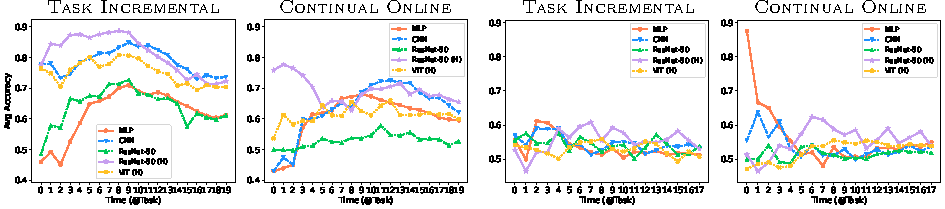
\includegraphics[width=1.0\textwidth]{imgs/kandy/Fig7.pdf}
	%\vskip -1mm
	\caption[Average accuracy over time on \textsc{KANDY-Induction-1}]{\textsc{KANDY-Induction-1} ({\it 1st, 2nd plot}) and \textsc{KANDY-Induction-2} ({\it 3rd, 4th plot}), average accuracy over time (i.e., after having processed data of each of the sequentially streamed tasks). {\it Left}: Task-incremental learning. {\it Right}: Continual online learning.}
	\label{kandy:fig:time_acc_easy_hard}
\end{figure}

\begin{figure}[!ht]
	\iffalse
	\centering  
	\includegraphics[width=0.75\textwidth, trim=0cm 1.1cm 0cm 0.0cm, clip]{fig/easy/independent-acc_matrix-test.pdf}\rotatebox[origin=c]{270}{\hskip -1.6cm \small \textsc{Independent}}\\
	\includegraphics[width=0.75\textwidth, trim=0cm 1.1cm 0cm 0.65cm, clip]{fig/easy/joint-acc_matrix-test.pdf}\rotatebox[origin=c]{270}{\hskip -1.8cm \small \textsc{Joint}}\\    
	\includegraphics[width=0.75\textwidth, trim=0cm 1.1cm 0cm 0.65cm, clip]{fig/easy/continual_task-acc_matrix-test.pdf}\rotatebox[origin=c]{270}{\hskip -1.8cm \small \textsc{Task Incr.}}\\
	\includegraphics[width=0.75\textwidth, trim=0cm 0.2cm 0cm 0.65cm, clip]{fig/easy/continual_online-acc_matrix-test.pdf}\rotatebox[origin=c]{270}{\hskip -2.7cm \small \textsc{Cont. Online}}\\
	\includegraphics[width=0.75\textwidth, trim=0cm 0.2cm 0cm 0.2cm, clip]{fig/sym_easy/independent-Accuracy.pdf}\rotatebox[origin=c]{270}{\hskip -2.7cm \small \textsc{Symbolic}}\\      
	\fi
	\centering
	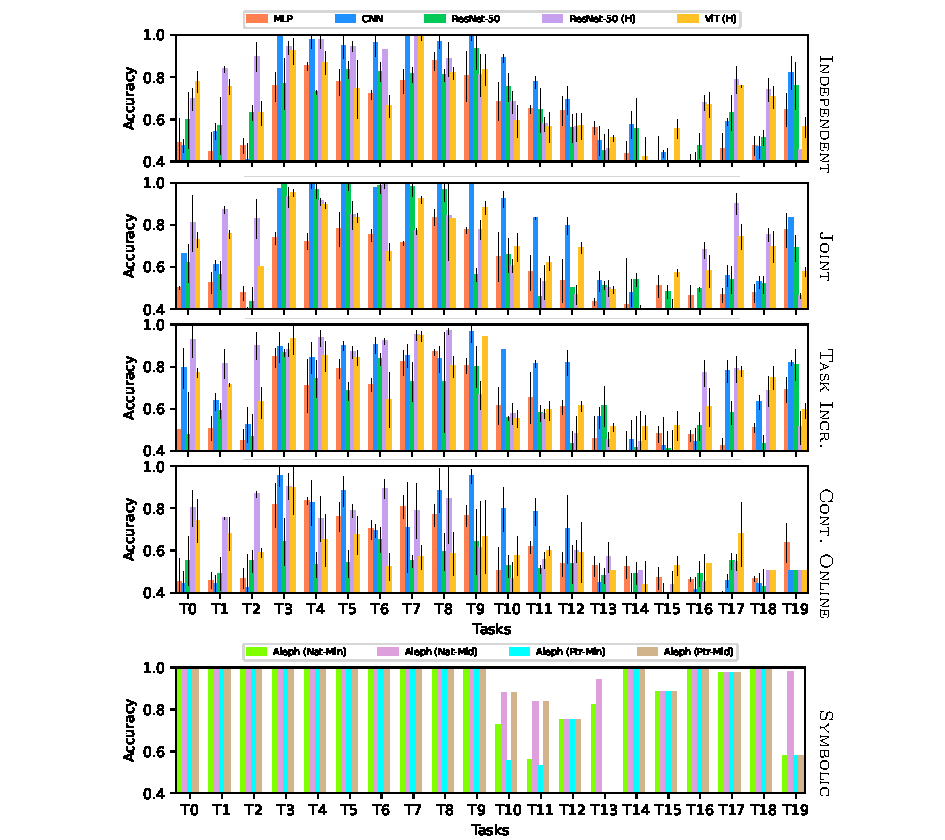
\includegraphics[width=1.0\textwidth]{imgs/kandy/Fig8.pdf}
	%\vskip -1mm
	\caption[Per-task accuracies over time on \textsc{KANDY-Induction-1}]{\textsc{KANDY-Induction-1}, per-task accuracies of the compared models in different learning settings. Neural (first four rows) and symbolic methods (last row) are represented with different colormaps. Models significantly under-performing (below 0.4) are not shown.}
	\label{kandy:fig:acc_per_task_easy}
\end{figure}

\begin{figure}
	\iffalse
	\centering
	\hskip -0.3cm \includegraphics[height=0.205\textwidth]{fig/easy/continual_task-avg_forgetting-test-time.pdf}
	\includegraphics[height=0.205\textwidth]{fig/easy/continual_task-backward_transfer-test-time.pdf}  
	\includegraphics[height=0.205\textwidth]{fig/easy/continual_task-forward_transfer-test-time.pdf}
	\rotatebox{270}{\hskip -2.4cm \small \textsc{Task Incr.}}\\
	\hskip -0.3cm \includegraphics[height=0.205\textwidth]{fig/easy/continual_online-avg_forgetting-test-time.pdf} 
	\includegraphics[height=0.205\textwidth]{fig/easy/continual_online-backward_transfer-test-time.pdf}
	\includegraphics[height=0.205\textwidth]{fig/easy/continual_online-forward_transfer-test-time.pdf}
	\rotatebox{270}{\hskip -2.6cm \small \textsc{Cont. Online}}\\
	\fi
	\centering
	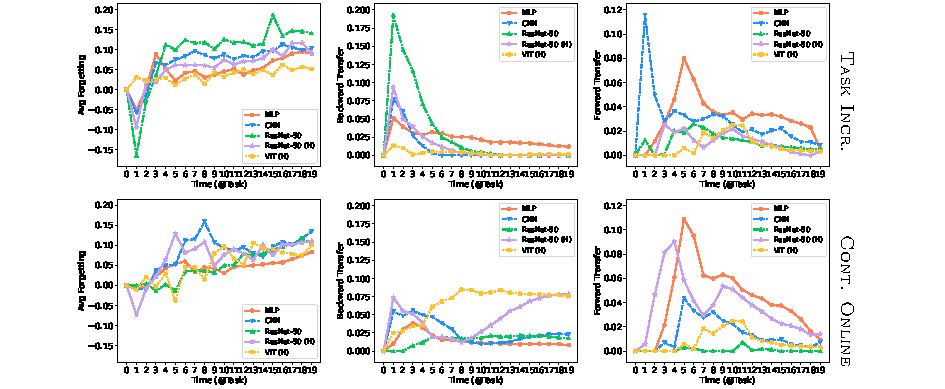
\includegraphics[width=1.0\textwidth]{imgs/kandy/Fig9.pdf}
	%\vskip -1mm
	\caption[Average forgetting over time on \textsc{KANDY-Induction-1}]{\textsc{KANDY-Induction-1}, average forgetting (the lower the better), backward transfer, forward transfer over time (i.e., after having processed data of each of the sequentially streamed tasks). {\it Top}: Task-incremental learning. {\it Bottom}: Continual online learning.}
	\label{kandy:fig:time_easy}
\end{figure}

\begin{figure}[!ht]
	\iffalse
	\centering
	\includegraphics[width=0.75\textwidth, trim=0cm 1.1cm 0cm 0.0cm, clip]{fig/hard_smaller/independent-acc_matrix-test.pdf}\rotatebox[origin=c]{270}{\hskip -1.6cm \small \textsc{Independent}}\\
	\includegraphics[width=0.75\textwidth, trim=0cm 1.1cm 0cm 0.65cm, clip]{fig/hard_smaller/joint-acc_matrix-test.pdf}\rotatebox[origin=c]{270}{\hskip -1.8cm \small \textsc{Joint}}\\    
	\includegraphics[width=0.75\textwidth, trim=0cm 1.1cm 0cm 0.65cm, clip]{fig/hard_smaller/continual_task-acc_matrix-test.pdf}\rotatebox[origin=c]{270}{\hskip -1.8cm \small \textsc{Task Incr.}}\\
	\includegraphics[width=0.75\textwidth, trim=0cm 0.2cm 0cm 0.65cm, clip]{fig/hard_smaller/continual_online-acc_matrix-test.pdf}\rotatebox[origin=c]{270}{\hskip -2.7cm \small \textsc{Cont. Online}}\\
	\includegraphics[width=0.75\textwidth, trim=0cm 0.2cm 0cm 0.2cm, clip]{fig/sym_hard/independent-Accuracy.pdf}\rotatebox[origin=c]{270}{\hskip -2.7cm \small \textsc{Symbolic}}\\ 
	\fi
	\centering
	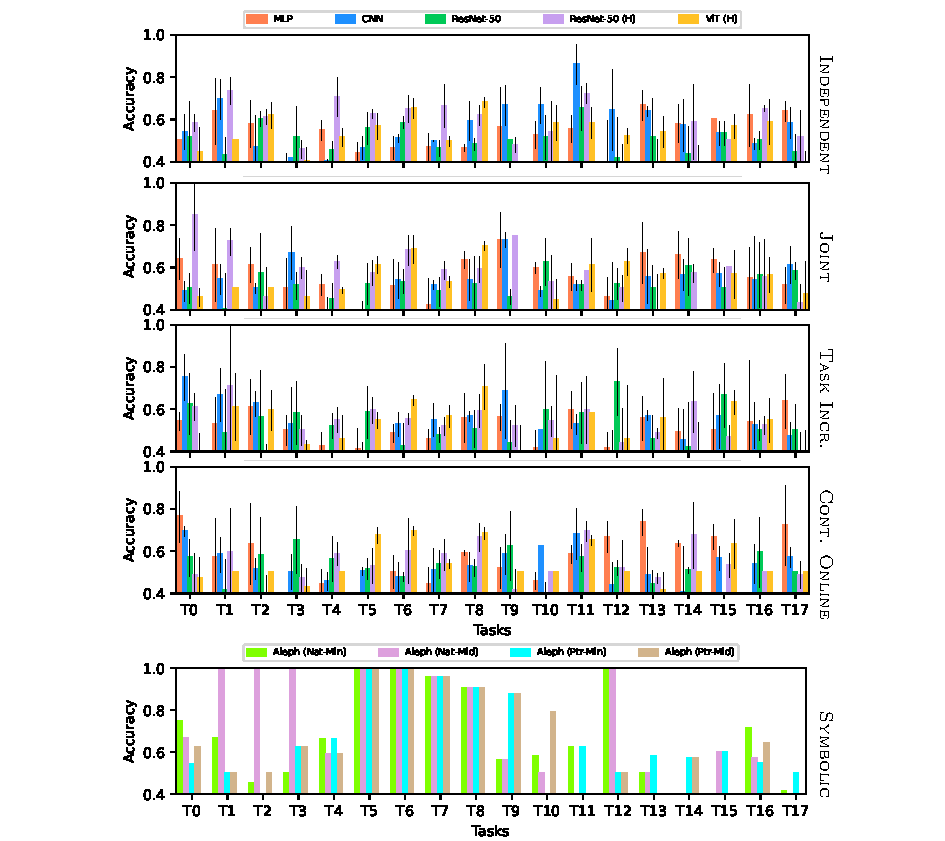
\includegraphics[width=1.0\textwidth]{imgs/kandy/Fig10.pdf}
	\caption[Per-task accuracies over time on \textsc{KANDY-Induction-2}]{\textsc{KANDY-Induction-2}, per-task accuracies of the compared models in different learning settings. Neural (first four rows) and symbolic methods (last row) are represented with different colormaps. Models significantly under-performing (below 0.4) are not shown.}
	\label{kandy:fig:acc_per_task_hard}
\end{figure}

\begin{figure}
	\iffalse
	\centering
	\hskip -0.2cm \includegraphics[height=0.24\textwidth]{fig/hard_smaller/continual_task-avg_forgetting-test-time.pdf}
	\includegraphics[height=0.24\textwidth]{fig/hard_smaller/continual_task-backward_transfer-test-time.pdf}  
	\includegraphics[height=0.24\textwidth]{fig/hard_smaller/continual_task-forward_transfer-test-time.pdf}
	\rotatebox{270}{\hskip -2.4cm \small \textsc{Task Incr.}}\\
	\hskip -0.2cm \includegraphics[height=0.24\textwidth]{fig/hard_smaller/continual_online-avg_forgetting-test-time.pdf} 
	\includegraphics[height=0.24\textwidth]{fig/hard_smaller/continual_online-backward_transfer-test-time.pdf}
	\includegraphics[height=0.24\textwidth]{fig/hard_smaller/continual_online-forward_transfer-test-time.pdf}
	\rotatebox{270}{\hskip -2.6cm \small \textsc{Cont. Online}}\\
	\fi
	\centering
	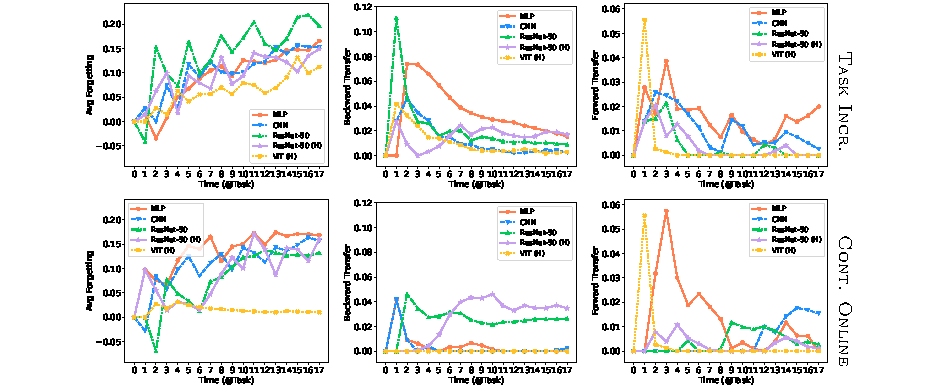
\includegraphics[width=1.0\textwidth]{imgs/kandy/Fig11.pdf}
	%\vskip -1mm
	\caption[Average forgetting over time on \textsc{KANDY-Induction-2}]{\textsc{KANDY-Induction-2}, average forgetting (the lower the better), backward transfer, forward transfer over time (i.e., after having processed data of each of the sequentially streamed tasks). {\it Top}: Task-incremental learning. {\it Bottom}: Continual online learning.}
	\label{kandy:fig:time_hard}
\end{figure}

\section{Results on \textsc{KANDY-Induction-1}}
\paragraph{Neural Experiments.}
% AVERAGE ACCURACY - COMPARING MODELS
Table~\ref{kandy:tab:acc_easy_hard} ({\it top}) reports the {\sc\small Average Accuracy} on test data at the end of learning. Neural Networks, overall, reach a maximum performance of $0.74$, with a preference for the convolutional models, either simple architectures trained from scratch ({\small\sc CNN}) or deeper pre-trained nets ({\small\sc ResNet-50 (H)}). The latter were pre-trained on data which is significantly different from \textsc{KANDY}, but they can still exploit their feature extraction skills to yield improvements with respect to their non-pre-trained counterpart ({\small\sc ResNet-50}). As expected, {\sc\small MLP} struggles to generalize to the \textsc{KANDY} test data, where shapes can be located in areas that are significantly different from the training ones, and where spatially pooled convolutional models are more appropriate. An aggressive spatial pooling can also limit the discrimination skills, this is what happens in {\sc\small ResNet-50} (both), where the final pooling yields a $1\times 1$ spatial map, while {\sc\small CNN} pools toward a $5\times 5$ representation which, for example, allows the final fully connected layers to discriminate what is on the left/right/up/bottom side of the image. Overall, {\sc\small ViT (H)} transformers are not far from convolutional models. 
In three out of five cases, training in a {\sc\small Joint} multi-task manner, improves the results, even though margin is small. This suggests that information sharing among tasks is not strongly promoted, or that the information in each task-data is enough to learn those properties shared among tasks. 
Interestingly, training in a continual manner ({\sc\small Task-incremental}) leads to results that are on par or even better than the other settings, and the temporal dynamics of the accuracy, reported in Figure~\ref{kandy:fig:time_acc_easy_hard} ({\it left}), shows somewhat limited drops over time, actually increasing up to half of the time axis (roughly). On one hand, this might either reinforce the hypothesis that there is limited information sharing, and that the network capacity is enough to learn the tasks without much forgetting-prone interference. On the other hand, this might also suggest a different scenario, in which there is indeed a positive sharing of information that does not trigger any forgetting of older, non-shared, information. 
To better explore this point, the dynamics of \textsc{Average Forgetting}, \textsc{Backward Transfer} and \textsc{Forward Transfer} over time are reported in Figure~\ref{kandy:fig:time_easy}, confirming an overall limited, but not negligible, level of forgetting. In particular, during the first time instants we observe positive backward and forward transfers of information, suggesting that the first tasks allow the networks to develop initial basic skills that are shared with the other tasks, while after a few time instants this does not happen anymore, suggesting a lower sharing of information (in both senses). %
As expected, the more challenging {\sc\small Continual online} setting is the one in which there is most room for improvement, since a single-pass on the data yields more difficulties to memorize the basic features of the tasks (results are $\approx 10\%$ lower than the other setting).
% 
Figure~\ref{kandy:fig:acc_per_task_easy} reports per-task accuracies. Overall, the first three tasks are tackled with an accuracy close or above $0.80$ only by a few models, while tasks from $4$ to $10$ are the ones on which many neural models perform well; networks incur in more difficulties in tasks from $11$ to $19$, among which the last three ones look less challenging than the others. Although with different absolute scores, each learning settings shows similar distribution of accuracies.

\paragraph{Symbolic Experiments.}
We report in Table~\ref{kandy:tab:acc_easy_hard} ({\it top}) the results obtained by Aleph on \textsc{KANDY-Induction-1} with the different combinations of knowledge bases. We note how the average test-accuracy is better than those obtained by neural approaches, which is not surprising as Aleph is provided with the correct symbolic representations of each image (as if the perception phase had been perfectly solved). Nevertheless, even in this setting some of the tasks result to be complex, especially with the \textsc{Minimal} knowledge base. We also report in Table~\ref{kandy:tab:symbolic_results} additional results describing the learned theories (\textsc{number of correct clauses}, \textsc{rule precision}, \textsc{recall}, \textsc{compression ratios}), to more specifically deepen the quality evaluation of such theories. In particular, all the implementations of Aleph are able to learn the correct clause(s) in the ground truth for 13 out of 20 tasks, thus leaving space for improvement. Moreover, we see that the average of per-task recall and per-task precision of the learned rules are both always above 0.85, so that the learned rules (on average) cover almost the total of positive examples, while producing few false positives.
%
Finally, the compression ratio between the number of clauses in the ground truth $C_{gt}$ (respectively, literals $L_{gt}$) and that in the learned theory $C_{\ell t}$ (respectively, $L_{\ell t}$) is frequently $< 1$, indicating an induced theory that is larger than the ground truth, thus a redundant (suboptimal) solution.

\section{Results on \textsc{KANDY-Induction-2}}
\paragraph{Neural Experiments.}
\textsc{KANDY-Induction-2} is composed of tasks that are significantly harder to solve by neural models, as shown in Table~\ref{kandy:tab:acc_easy_hard} ({\it middle}). The top-accuracy is $0.59$, thus not far from a random guess, making it hard to trace strong conclusions on the comparisons among the different models/settings. 
In this case, {\sc\small Continual online} learning is not different from the multiple-epochs {\sc\small Task-incremental} setting, confirming that multiple passes on the data are not enough to introduce significant improvements. %The temporal dynamics, as shown in 
Figure~\ref{kandy:fig:time_acc_easy_hard} ({\it right}) reports similar temporal dynamics, with the exception of {\sc\small MLP} in {\sc\small Continual online}, that is able to reach high accuracy on the first task and then incur in evident drops over time. 
The dynamics of forgetting and forward transfer, shown in Figure~\ref{kandy:fig:time_hard}, are similar to \textit{KANDY-Induction-1}. {\sc\small ViT (H)} seems to experience almost no forgetting, but this phenomenon is caused by accuracy scores too close to random guessing. The backward transfer is more evident on the long run, compared to \textsc{KANDY-Induction-1}, while it is less effective in the first time instants, showing an intrinsically more complicated capability of sharing information, due to the difficulty of the tasks, leaving room to novel research. 
Per-task accuracies are reported in Figure~\ref{kandy:fig:acc_per_task_hard}. Tasks $1$, $2$, $9$, and $11$ are the ones on which neural models perform slightly better. 
%
We performed additional experiments with a larger version of \textsc{KANDY-Induction-2} ($1000$ samples per task, fully supervised), reporting results in Table~\ref{kandy:tab:acc_easy_hard} ({\it bottom}), to assess whether there is room for improvement with additional data. We observe improvements in terms of accuracy, that are coherent with the overall picture discussed for \textsc{KANDY-Induction-1}. This confirms that the benchmark is very challenging and neural models in Continual Learning settings struggle more than in the simpler case of \textsc{KANDY-Induction-1}. 

\paragraph{Symbolic Experiments.}
Table~\ref{kandy:tab:acc_easy_hard} ({\it middle}) reports the results obtained by Aleph on \textsc{KANDY-Induction-2}. Even though Aleph is given correct symbolic representations of each image, most of the tasks still remain extremely challenging. The statistics reported in Table~\ref{kandy:tab:symbolic_results} ({\it bottom}) highlight that only for a few (3 to 6) of the 18 tasks, the correct solution is induced. The learned theories typically contain many clauses (low ratio $C_{gt} / C_{\ell t}$) specialized and covering few cases (higher precision than recall), and manual inspection revealed the presence of ``overfitting'' facts in the form \texttt{valid(training\_sample)}, which inflate the $C_{gt} / C_{\ell t}$ ratio without improving performance. Slightly better performance can be observed with \textsc{Natural} encoding rather than \textsc{Ptr}, and with \textsc{Mid} knnowledge base with respect to \textsc{Minimal}: the number of correct tasks is higher and both compression ratios are closer to 1. 
%not only the number of correct tasks is higher, but also the compression ratios (for both clauses and literals) is closer to 1 
While this can be in part attributed to encodings other than \textsc{Nat-Mid} requiring longer clauses for the same concept, low compression ratios on \textsc{Nat-Mid} hint at a generalized difficulty in inducing effective clauses. Overall, these results confirm that \textsc{KANDY-Induction-2} is extremely challenging even for symbolic methods with a non-noisy knowledge base.


\section{Vision Language Models Experiments}\label{kandy:sec:bongard}
\begin{table}[t]
	\centering
	\resizebox{\textwidth}{!}{
		\begin{tabular}{lrrrr}
			\toprule
			& \footnotesize \sc LLaVA & \footnotesize \sc MoE-LLaVA & \footnotesize \sc InternLM-XComposer & \footnotesize \sc Human\\
			\midrule
			\footnotesize \textsc{Absence of ``bad'' tokens} & 1/20 & 6/20 & 2/20 & 20/20 \\
			\footnotesize \textsc{At least one ``good'' token} & 4/20 & 9/20 & 13/20 & 20/20 \\
			\footnotesize \textsc{Did not respond} & 4/20 & 0/20 & 0/20 & 0/20 \\
			\footnotesize \textsc{Recurring hallucinations} & 15/20 & 7/20 & 0/20 & 0/20 \\
			\footnotesize \textsc{Novel hallucinations} & 1/20 & 3/20 & 14/20 & 0/20 \\
			\bottomrule
		\end{tabular}
	}
	\caption[Vision Language Models experiments on \textsc{KANDY-Bongard-1}]{Qualitative statistics on Vision Language Models experiments. Recurring hallucinations are  ``grid pattern'',  ``same color'' and ``three objects on the left''.}
	\label{kandy:tab:bongard}
\end{table}
%Tasks in KANDY can also be framed as Bongard problems, and presented to VLMs to assess their visual reasoning capabilities.
We run zero-shot experiments on \textsc{KANDY-Bongard-1} to assess abstract reasoning capabilities of Vision Language Models, selecting representatives of three families: (i.) vanilla \textsc{LLaVA}~\cite{liu2024visual}, (ii.)  \textsc{MoE-LLaVA}~\cite{lin2024moe}, and (iii.)  \textsc{InternLM-XComposer}~\cite{zhang2023internlm}.
For each model, we perform inference exploiting the Hugging Face Spaces platform,\footnote{\url{https://huggingface.co/spaces}} to run inference on ready-to-use checkpoints.\footnote{\textsc{LLaVA}: \url{https://huggingface.co/spaces/badayvedat/LLaVA}, \textsc{MoE-LLaVA}: \url{https://huggingface.co/spaces/LanguageBind/MoE-LLaVA}, \textsc{InternLM-XComposer}: \url{https://huggingface.co/spaces/Willow123/InternLM-XComposer}}
Each experiment is run with the Space's default hyper-parameters, providing a Foundalis-style image,\footnote{This is a standard format for Bongard problems.} along with the first prompt of Figure~\ref{kandy:fig:prompts} (Appendix~\ref{app:bongard}). If the Vision Language Model does not respond with an answer based on the image content (e.g., because it paraphrases the input prompt), we allow a second answer by adding the second prompt of Figure \ref{kandy:fig:prompts} (Appendix~\ref{app:bongard}) to the conversation.
\begin{tcolorbox}[breakable,enhanced jigsaw,opacityback=0,]
	\centering
	\footnotesize
	\begin{dialogue}
		\speak{LLaVA} The image consists of twelve panels, each containing atomic objects characterized by shape, color, and size. The panels on the left share a common property, while the panels on the right violate that property.
		
		One possible property that the left panels share is that all the objects within each panel have the same color. This can be inferred from the fact that the left panels contain only one color each, and all the objects within each panel have the same color.
		
		On the other hand, the panels on the right violate this property by containing objects with different colors. This can be observed by the presence of multiple colors in each of the right panels.
		
		Therefore, the property that the left panels share is that all the objects within each panel have the same color, while the panels on the right violate this property by containing objects with different colors.
		%\vspace{1em}
		%    \speak{MoE-LLaVA} \direct{Error}
		%\vspace{1em}
		%    \speak{InternLM-XComposer} The property depicted by the panels is a structural uniformity along the vertical axis. Specifically, each panel on the left side exhibits objects positioned around a vertical line:
		
		%In every left panel:
		
		%Objects are distributed equally along the vertical.
		%There are no gaps or overlaps between objects in horizontal alignment.
		
		%While the right set of panels breaks this structure by:
		
		%   Having varying object numbers and orientations at different heights.
		%   Violating the equal spacing along the vertical axis.
		
		%Hence the described property regards structured vertical alignment in each set of panels.
	\end{dialogue}
	%\captionof{figure}{Baseline responses when no image is provided.}
	%\label{kandy:fig:baseline}
\end{tcolorbox}
\noindent\begin{minipage}{\textwidth}
	%\vskip -2mm
	\captionof{figure}[LLaVA baseline response]{\textsc{LLaVA} baseline response when no image is provided.}\label{kandy:fig:baseline}
\end{minipage}
Tasks are presented in order (from \textsc{KANDY-Bongard-1} Task 0 to \textsc{KANDY-Bongard-1} Task 19), resetting the conversation history before each new image.
%\paragraph{Vision Language Models} 
Table \ref{kandy:tab:bongard} collects qualitative results for each task, compiled by analyzing each answer manually (the full transcript of each Vision Language Model experiment is included in Appendix~\ref{app:bongard}). Due to the intrinsic difficulty of establishing a decision boundary between correct and incorrect responses, we analyze the presence of ``good'' tokens (marked in green in subsequent figures), which are related to the ground truth rule, and the absence of ``bad'' tokens (in red), which correspond to an incorrect answer. We also count the number of answers containing hallucinations (descriptions of features not present in the image), regardless of their contribution to the final decision.
%
In general, \textsc{LLaVA} is the worst performing Vision Language Model on the presented Bongard problems, and it often responds by hallucinating one of three recurring properties (presence of grid patterns, three objects, and same color), or by paraphrasing the input prompt. \textsc{MoE-LLaVA} seems to be the most robust against hallucinations and incorrect features. Finally, \textsc{InternLM-XComposer} is both the best performing model, but also the most affected by hallucinations, which, unlike \textsc{LLaVA}, can take the form of a wide variety of features.
%
\begin{tcolorbox}[breakable,enhanced jigsaw,opacityback=0,]
	\footnotesize
	\centering
	%\begin{framed}
	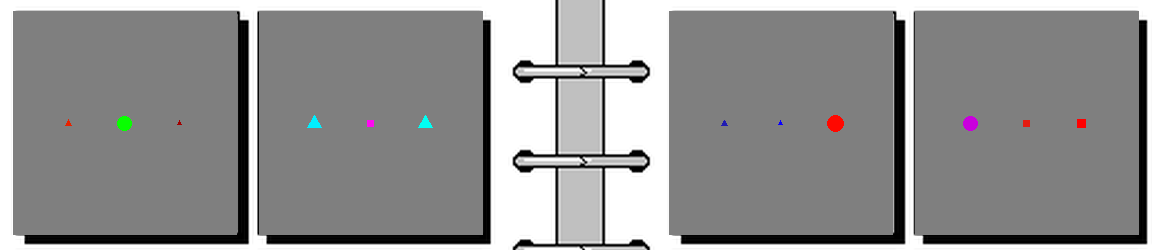
\includegraphics[width=.8\linewidth]{imgs/kandy/Fig5.png}\\
	\begin{dialogue}
		\speak{Prompt} \direct{Prompt}
		\speak{MoE-LLaVA}The property that the panels on the right side of the image violate is the color of the atomic objects. In the left half of the image, \textcolor{red}{all the atomic objects are of the same color}, while in the right half, the color of the objects varies. This difference in color is the distinguishing feature that helps identify the two halves of the image.
		
		\speak{Prompt}The answer is wrong, please correct it.
		
		\speak{MoE-LLaVA}I apologize for the mistake in my previous response. The property that the panels on the right side of the image violate is \textcolor{red}{the shape of the atomic objects}. In the left half of the image, all the atomic objects are of the same shape, while in the right half, the shape of the objects varies. This difference in shape is the distinguishing feature that helps identify the two halves of the image.
		
		\speak{Prompt}Are there any symmetries in the image?
		
		\speak{MoE-LLaVA}Yes, there are symmetries in the image. The panels on the left side of the image are symmetrically arranged, while the panels on the right side are not. This symmetry helps to visually distinguish the two halves of the image.
	\end{dialogue}    
	%\end{framed}
	%\captionof{figure}{Example of user-guided resolution of a Bongard problem (KANDY-Easy, task 14, ground truth: ``A palindrome of three objects'').}
	%\label{kandy:fig:user-guided-bongard}
\end{tcolorbox}
\noindent\begin{minipage}{\textwidth}
	%\vskip -2mm
	\captionof{figure}[User-guided Vision Language Model resolution on \textsc{KANDY-Bongard-1}]{Example of user-guided resolution of a Bongard problem (\textsc{KANDY-Bongard-1}, task 14, ground truth: ``A palindrome of three objects'', image cropped to the first four panels).}\label{kandy:fig:user-guided-bongard}
\end{minipage}
In addition, Figure~\ref{kandy:fig:baseline} presents the baseline output for \textsc{LLaVA}, when no input image is provided. The response highlights hallucinating behavior, with non-existent features being described. %With the exception of \textsc{MoE-LLaVA}, which does not return any output, possibly due to algorithmic checks before inference, models present hallucinating behavior, describing non-existent features.
Figure~\ref{kandy:fig:user-guided-bongard} represents user-guided reasoning capabilities of \textsc{MoE-LLaVA}, on one of the most difficult tasks of \textsc{KANDY-Bongard-1}. The Vision Language Model required three attempts of increasing helpfulness (original prompt, negative feedback, pointing the attention towards the relevant feature) in order to produce the correct response.
None of the models is capable of solving the same task (Figure~\ref{fig:task14-bongard} in Appendix~\ref{app:bongard}), when presented in a zero-shot setting (i.e., only the input prompt).
%Figures \ref{kandy:fig:task4-bongard}, \ref{kandy:fig:task8-bongard} and \ref{kandy:fig:task9-bongard} present three additional examples of zero-shot inference.
%Two VLMs out of three can solve Task 4 (Figure~\ref{kandy:fig:task4-bongard}), even though \textsc{InternLM-XComposer} hallucinates non-existing features. Task 8 (Figure~\ref{kandy:fig:task8-bongard}), which has roughly the same complexity as the previous one (all objects are yellow, instead of green), but a missing positive sample, yields radically different responses, with \textsc{LLaVA} identifying the correct rule (but hallucinating the color) and \textsc{InternLM-XComposer} producing an over-specified rule (yellow or magenta), after hallucinating a series of distracting features. \textsc{MoE-LLaVA}, on the other hand, produces a completely incorrect answer.
Tasks 0 to 8 are characterized by a single object for each panel and a trivial property (i.e., same shape or same color), however none of the Vision Language Models is capable of consistent behavior, with similar tasks eliciting highly different responses (cfr. Task 4 and Task 5, Figures \ref{fig:task13-bongard} and \ref{fig:task14-bongard}, respectively, in Appendix~\ref{app:bongard}). 
Task 9 (Figure~\ref{kandy:fig:task9-bongard}), which contains two objects for each panel, presents a challenge for every model. After paraphrasing the input prompt, \textsc{LLaVA} is capable of producing a correct, but incomplete, answer, while the other two models fail.

\begin{tcolorbox}[breakable,enhanced jigsaw,opacityback=0,]
	\footnotesize
	\centering
	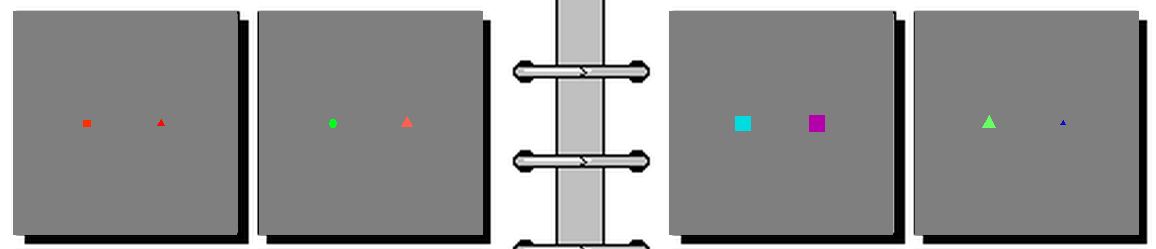
\includegraphics[width=.8\linewidth]{imgs/kandy/Fig6.png}\\
	\begin{dialogue}
		\speak{LLaVA} The image features twelve panels, each containing atomic objects characterized by shape, color, and size. [\dots]
		\\\direct{Did not answer.}
		\speak{LLaVA} After analyzing the image, it appears that \textcolor{red}{the atomic objects are arranged in a grid pattern}, with each panel containing a specific number of objects. [\dots]
		
		Upon closer examination, it can be observed that all objects in the left panels are \textcolor{ForestGreen}{triangles with a specific color}, while the objects in the right panels are squares with a different color. The property that unifies the panels on the left is the shape of the objects, which are all triangles. The property that differentiates the panels on the right is the color of the objects, which is different from the color of the objects in the left panels.
		
		In summary, the left panels share the property of \textcolor{ForestGreen}{having triangular objects with a specific color}, while the right panels violate this property by having square objects with a different color.
		\vspace{1em}
		\speak{MoE-LLaVA} The property that the panels on the right side of the image violate is the \textcolor{red}{color of the atomic objects}. All the panels on the left side of the image have objects with the same color, while the panels on the right side have objects with different colors. This difference in color is the main distinguishing feature between the two sets of panels.
		%\\\direct{Did not answer.}
		%\speak{MoE-LLaVa} 
		\vspace{1em}
		\speak{InternLM-XComposer} The panels have two distinct color arrangements.
		
		Property: \textcolor{red}{The upper halves of the images on the left need to follow a color grid pattern where each column follows another}. For instance, there are three columns in each panel.
		
		Violation: The same property does not apply to the lower halves.
		
		Let's work through this:
		
		All panels (ignoring any empty ones) contain 6 shapes and colors (2 triangles, 2 squares/blocks, and either 2 circles or 2 of one specific color circle).
		The first two columns form a 1x2 square (a horizontal arrangement where the blue circle is in row 1 and the large triangle is in row 3). The third column has a unique shape/color that differs from these two columns.
		
		Therefore, considering spatial relations and arrangement of objects, identify that for a consistent layout, similar color patterns should hold true but not in a grid pattern where each column is similar.
		%\\\direct{Did not answer.}
		%\speak{InternLM-XComposer} 
	\end{dialogue}
	%\captionof{figure}{KANDY-Easy,  Task 9: ``There is a red triangle on the right (two objects)''. Tokens in red correspond to incorrect features, tokens in green correlate with the correct answer.}
	%\label{kandy:fig:task9-bongard}
\end{tcolorbox}
\noindent\begin{minipage}{\textwidth}
	%\vskip -2mm
	\captionof{figure}[Zero-shot Vision Language Model resolution on \textsc{KANDY-Bongard-1} Task 9]{\textsc{KANDY-Bongard-1},  Task 9: ``There is a red triangle on the right (two objects)'', image cropped to the first four panels. Tokens in red correspond to incorrect features, tokens in green correlate with the correct answer.}\label{kandy:fig:task9-bongard}
\end{minipage}